\documentclass[12pt,a4paper]{article}
\usepackage[utf8]{inputenc}
\usepackage[T1]{fontenc}
\usepackage[french]{babel}
\usepackage{setspace}
\usepackage{geometry}
\usepackage{graphicx}
\usepackage{array}
\usepackage[hyphens]{url}
\usepackage[table]{xcolor}
\usepackage[colorlinks=true, linkcolor=black, urlcolor=blue, citecolor=blue]{hyperref}
\hypersetup{breaklinks=true,colorlinks=true,urlcolor=blue}
\Urlmuskip=0mu plus 2mu
\sloppy
\setlength{\emergencystretch}{3em}
\usepackage{float}

\geometry{margin=2.5cm}
\usepackage{fancyhdr}
\pagestyle{fancy}

\fancyhf{}
\fancyfoot[L]{\small CarryBot - Master 2 MIASHS, parcours HANDI}
\fancyfoot[R]{\thepage}

\renewcommand{\headrulewidth}{0pt}
\renewcommand{\footrulewidth}{0.4pt}

\begin{document}

\begin{titlepage}
\centering

\begin{center}
\begin{minipage}{0.36\textwidth}
  \centering
  
\includegraphics[width=0.75\linewidth]{../img/logo-p8.jpg}
\end{minipage}
\hfill
\begin{minipage}{0.45\textwidth}
  \centering
  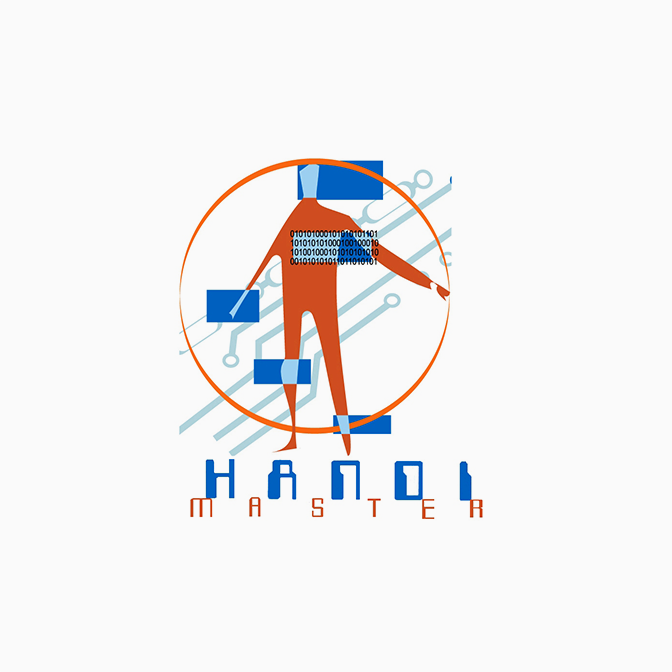
\includegraphics[width=0.5\linewidth]{../img/logo-handi.png}
\end{minipage}
\end{center}

\vspace*{1.5cm}

{\Large \textbf{Master 2 MIASHS - Parcours Technologie \& Handicap}}\\[0.3cm]
{\large Université Paris 8, Vincennes - Saint-Denis}\\[2.2cm]

{\LARGE \textbf{CarryBot}\\[0.2cm]
\Large \textbf{Robot compagnon d’assistance pour transport d’objets légers en intérieur}}\\[1.5cm]
% -------------------------------------------------------------
% Logo / visuel CarryBot (page de garde)
% -------------------------------------------------------------
\begin{figure}[H]
    \centering
    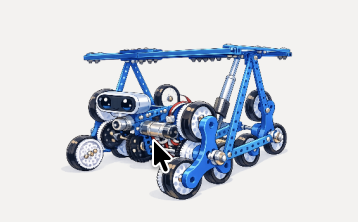
\includegraphics[width=0.38\textwidth]{../img/carryBot.png} % <- mets ta photo ici
\end{figure}
\vspace{0.5cm}

\begin{flushleft}
\begin{minipage}{0.55\textwidth}
\textbf{Rédigé par:}\\[0.2cm]
Lena BESSA\\
Zhaoyu WANG\\
Xinqi TANG\\
Lou LOPEZ\\[1.5cm]
\end{minipage}
\begin{minipage}{0.40\textwidth}
\textbf{Enseignants:}\\[0.2cm]
Dominique ARCHAMBAULT\\
Salvatore ANZALONE\\[1.2cm]
\end{minipage}

\vspace*{1.2cm}

\textbf{Année universitaire:} 2025-2026
\end{flushleft}

\end{titlepage}

\newpage

% -------------------------------------------------------------
% TABLE DES MATIERES
% -------------------------------------------------------------
\tableofcontents
\newpage

% -------------------------------------------------------------
% TABLE DES FIGURES
% -------------------------------------------------------------
\listoffigures
\addcontentsline{toc}{section}{Table des figures}

\newpage

% -------------------------------------------------------------
% GLOSSAIRE
% -------------------------------------------------------------
\section*{Glossaire}
\addcontentsline{toc}{section}{Glossaire}

\begin{table}[H]
\centering
\renewcommand{\arraystretch}{1.4}
\begin{tabular}{|p{4cm}|p{11cm}|}
\hline
\textbf{Terme} & \textbf{Description} \\ \hline

Tri-Star & Mécanisme composé de trois roues montées sur un même moyeu rotatif, permettant le franchissement de petites marches ou obstacles. \\ \hline

IMU &  (Inertial Measurement Unit) Capteur regroupant accéléromètre, gyroscope et parfois magnétomètre, servant à mesurer l’inclinaison, l’accélération et la rotation du robot. \\ \hline

Raspberry Pi 5 & Micro-ordinateur monocarte utilisé comme unité centrale embarquée pour la gestion des capteurs, moteurs et communications du robot. \\ \hline

Intel RealSense D435 & Caméra de profondeur permettant de capturer une carte 3D de l’environnement, utilisée pour la perception et la détection avancée. \\ \hline

Vérin linéaire & Actionneur électrique convertissant une rotation en mouvement linéaire, utilisé ici pour stabiliser la palette et ajuster son inclinaison. \\ \hline

SLAM & Acronyme de “Simultaneous Localization And Mapping”, méthode avancée de navigation exclue du périmètre de ce prototype. \\ \hline

LIDAR & Capteur de télémétrie laser utilisé pour la cartographie de l’environnement, proposé en perspective future. \\ \hline

PMR  & Personne à Mobilité Réduite \\ \hline

RGAA & Référentiel Général d’Accessibilité pour les Administrations, norme française d’accessibilité numérique applicable à l’application mobile. \\ \hline

\end{tabular}
\end{table}
\newpage
% -------------------------------------------------------------
% 1. PRÉSENTATION DU PROJET
% -------------------------------------------------------------
\section{Présentation du projet}

\subsection{Éléments généraux du projet}

\subsubsection{Contexte}
CarryBot s’inscrit dans un projet académique visant à explorer la robotique mobile d’assistance au sein d’environnements intérieurs contrôlés. 
Dans le cadre d’un enseignement universitaire, le robot constitue un support de travail permettant d’aborder la mécatronique, les technologies embarquées et les problématiques d’accessibilité.  
Le projet s’appuie sur une démarche de conception centrée utilisateur afin d’illustrer comment une solution robotique peut répondre à des besoins concrets d’aide au transport d’objets.

\subsubsection{Objectif général}
L’objectif principal est de développer un prototype fonctionnel de robot capable de transporter des objets légers de manière sécurisée et accessible.  
Ce prototype doit démontrer la faisabilité d’un système simple, robuste et compréhensible, utilisable à des fins domestique et médico.

\subsubsection{Finalités du projet}

Les finalités du projet CarryBot s’inscrivent dans une démarche d’assistance aux publics fragiles en environnement intérieur. Elles se déclinent comme suit:

\begin{itemize}
    \item \textbf{Soutien aux personnes à mobilité réduite:} faciliter le transport d’objets du quotidien pour des utilisateurs présentant un handicap moteur ou une autonomie limitée.
    
    \item \textbf{Allègement de la charge physique des aidants:} réduire les déplacements répétitifs du personnel soignant ou des aidants dans des environnements tels que les hôpitaux, centres de rééducation ou EHPAD.
    
    \item \textbf{Assistance aux personnes âgées:} proposer un dispositif aidant au transport d’objets dans un espace sécurisé, limitant les risques liés aux efforts ou aux déplacements non adaptés.
    
    \item \textbf{Amélioration de l’autonomie en intérieur:} offrir un robot capable de fonctionner dans des espaces maîtrisés (chambre, couloir, domicile adapté) afin de soutenir un maintien de l’autonomie au quotidien.
    
    \item \textbf{Accessibilité et simplicité d’usage:} fournir une interface de pilotage intuitive, basée sur des pictogrammes, utilisable par des personnes présentant des limitations motrices ou cognitives.
    
\end{itemize}


\subsubsection{Population concernée}

CarryBot s’adresse prioritairement à des publics nécessitant une assistance au transport d’objets dans un environnement intérieur. Les principales populations concernées sont:

\begin{itemize}
    \item des personnes en situation de handicap moteur
    \item des personnes âgées
    \item des patients
    \item des aidants et personnels soignants
    \item des structures médico-sociales EHPAD, foyers de vie, services de rééducation.
\end{itemize}

% -------------------------------------------------------------
% 1.X ORGANISATION DU PROJET
% -------------------------------------------------------------

\subsection{Organisation du projet}

\subsubsection{Éléments de macro-planning}
Le déroulement du projet suit les jalons suivants:
\begin{figure}[h!]
    \centering
    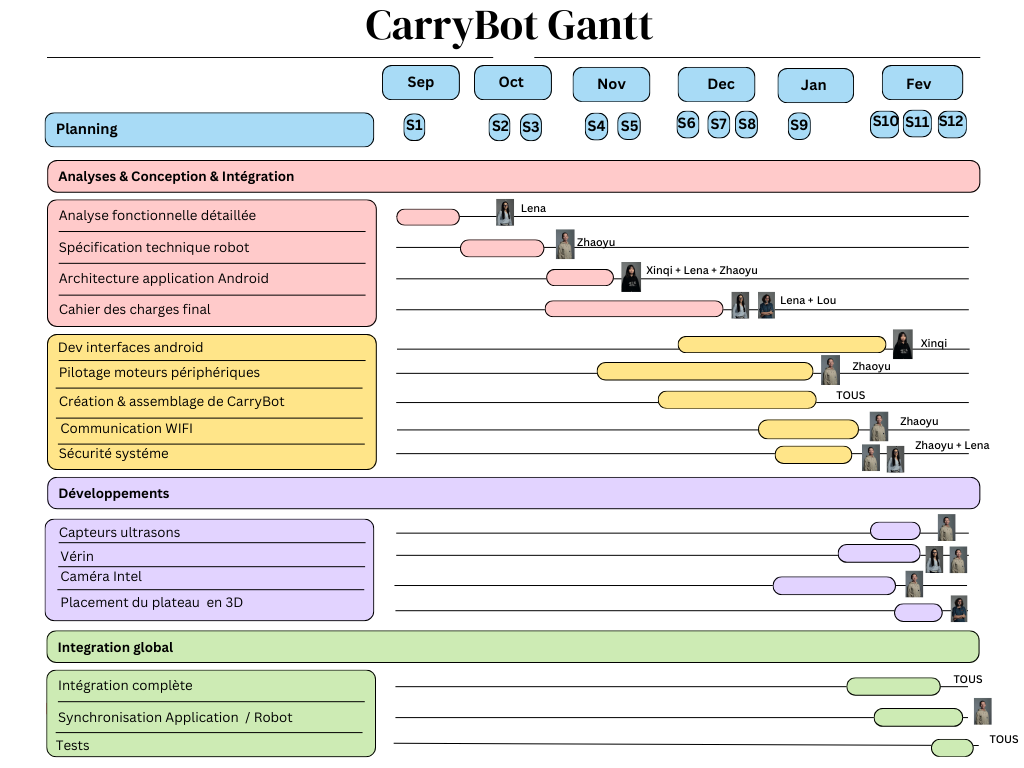
\includegraphics[width=1.10\linewidth]{../img/GANTT-CarryBot.png}
    \caption{Diagramme de Gantt du projet CarryBot}
    \label{fig:architecture_carrybot}
\end{figure}

\subsubsection{Répartition des rôles au sein de l’équipe}

\begin{tabular}{|p{4cm}|p{11cm}|}
\hline
\textbf{Membre} & \textbf{Responsabilités principales} \\ \hline

Lena Bessa & Rédaction du cahier des charges (format LaTeX), analyse des besoins, élaboration des scénarios d’usage, contribution à la conception fonctionnelle et ergonomique. \\ \hline

Zhaoyu Wang & Modélisation 3D du système Tri-Star, sélection et analyse des solutions matérielles (Raspberry Pi, capteurs), participation à la conception technique. \\ \hline

Xinqi Tang & Développement de l’application Android, intégration des fonctionnalités d’accessibilité, contribution à l’architecture logicielle. \\ \hline

Lou Lopez & Réalisation de l’état de l’art, recherche documentaire, veille technologique et participation à la conception globale du projet. \\ \hline

\end{tabular}

\vspace{0.6cm}

% -------------------------------------------------------------
% 2. ETUDE DE L’EXISTANT
% -------------------------------------------------------------
\section{État de l’art}

\subsection{L’usage des robots en milieu clinique et au quotidien}

Face au vieillissement rapide de la population mondiale et à la pénurie croissante de ressources médicales, le développement de la robotique dans le secteur de la santé apparaît comme une réponse structurante \cite{bloss2011}. Cette transition a été accélérée par la pandémie de COVID-19, qui a renforcé les enjeux de distanciation sociale et les besoins de téléprésence \cite{bourdon2023}.

\subsubsection*{Robotique en milieu clinique}

Cette section s’appuie sur trois revues de littérature: (1) une revue systématique centrée soins critiques \cite{teng2022}, (2) un survey sur les robots infirmiers intelligents \cite{wang2024}, et (3) une revue de systèmes robotiques de santé \cite{holland2021}. Un constat transversal ressort: au-delà de la téléprésence et de certains actes à distance, l’un des leviers majeurs concerne la \textbf{logistique hospitalière}, notamment la distribution de médicaments et le transport de consommables, dans un contexte de surcharge de travail et de sous-effectif.\\

Le robot \textbf{TUG} (Aethon), développé dès 2004, constitue un système emblématique, largement documenté \cite{holland2021,teng2022}. Il s’agit d’un robot mobile autonome capable de transporter médicaments, sang, nourriture, linge ou déchets, avec une forte capacité d’emport. Il s’appuie sur des plans numériques, des capteurs (laser/ultrasons) pour l’évitement d’obstacles, et peut interagir avec l’infrastructure (ex. ascenseurs) via réseau sans fil \cite{holland2021}. Les chaînes de traitement en pharmacie peuvent ainsi être automatisées via programmation de séquences de livraison, réduisant le temps de cycle et libérant du temps opérateur \cite{teng2022}.\\
\begin{figure}[H]
    \centering
    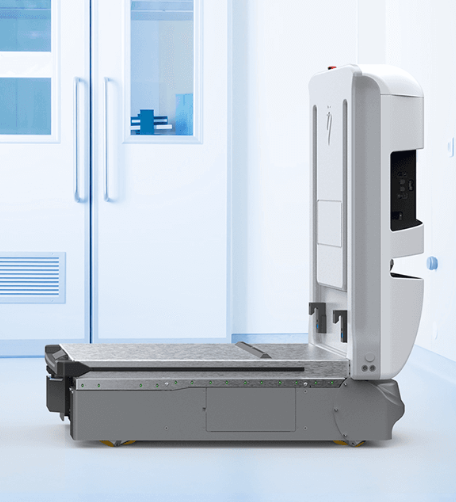
\includegraphics[width=0.45\linewidth]{../img/tug.png}
    \caption{Robot logistique hospitalier TUG (Aethon)}
    \label{fig:tug}
\end{figure}

D’autres systèmes mettent l’accent sur des exigences spécifiques: sécurisation anti-vol et anti-manipulation non autorisée (HOSPI de Panasonic) \cite{holland2021}, maintien thermique pour les repas (prototype i-MERC) \cite{holland2021}, transport de matériel stérile (MiR100) \cite{holland2021}. Enfin, \textbf{Moxi} vise l’assistance aux infirmières (récupération de fournitures, EPI) avec base mobile, navigation et évitement d’obstacles ; certaines versions intègrent un bras pour manipuler des objets \cite{wang2024}.

\subsubsection*{Robotique d’assistance à domicile}

La robotique d’assistance vise l’autonomie et le maintien à domicile, particulièrement pour les personnes âgées et les personnes à mobilité réduite. Plusieurs dispositifs de service sont rapportés, offrant des fonctionnalités de \textbf{rappels de médicaments}, d’appels, de divertissement et de petites commissions \cite{wang2024}. Le robot \textbf{Care-O-Bot} constitue une ligne de recherche historique: ses versions successives illustrent une montée en complexité (mobilité, capteurs, interface tactile, bras motorisés) et un positionnement orienté interaction et acceptabilité sociale \cite{graf2009,kittmann2015,graf2023}.\\
\begin{figure}[H]
    \centering
    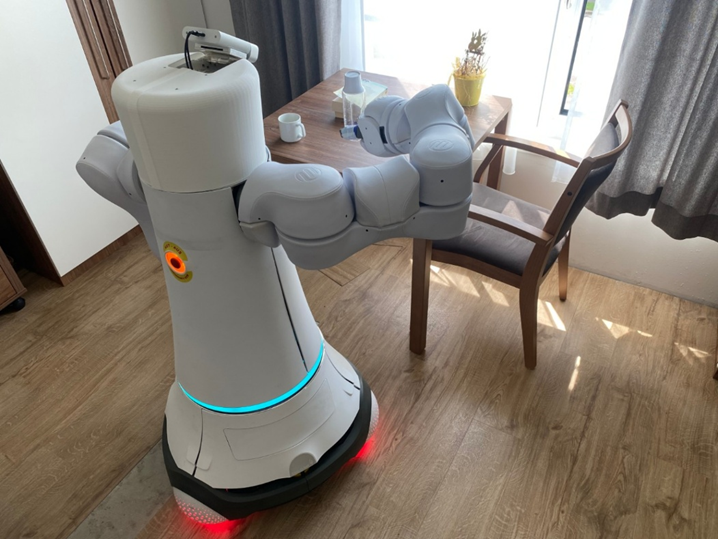
\includegraphics[width=0.45\linewidth]{../img/care-o-bot.png}
    \caption{Care-O-Bot – Robot d’assistance domestique}
    \label{fig:careobot}
\end{figure}

En complément des dispositifs de recherche, des solutions plus récentes existent sur le marché, comme le \textbf{Labrador Retriever}, robot domestique capable de naviguer dans un logement, de transporter des charges et d’être commandé vocalement (Alexa). Enfin, des robots ciblent le transport vertical de charges moyennes (ex. \textbf{ROSA}), orientés franchissement d’escaliers avec usage logistique domestique.

\begin{figure}[H]
    \centering
    \begin{minipage}{0.47\linewidth}
        \centering
        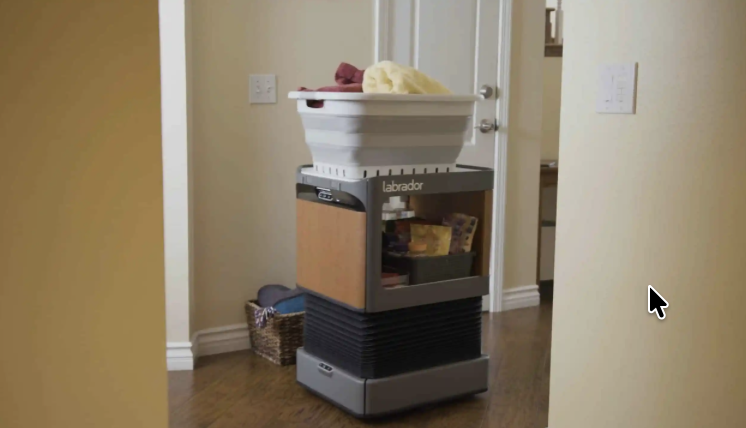
\includegraphics[width=\linewidth]{../img/labrador.png}
        \caption{Labrador Retriever}
        \label{fig:labrador}
    \end{minipage}
    \hfill
    \begin{minipage}{0.42\linewidth}
        \centering
        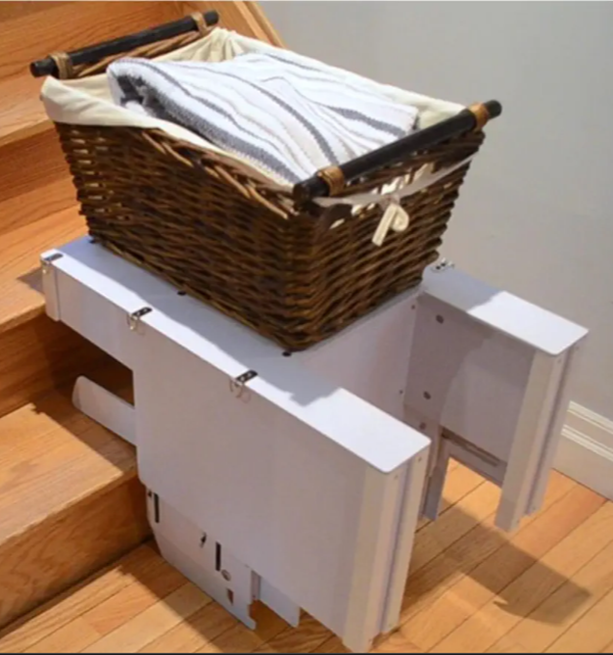
\includegraphics[width=\linewidth]{../img/rosa.png}
        \caption{ROSA }
        \label{fig:rosa}
    \end{minipage}
\end{figure}
%--------------------------------------------------------------
\subsubsection*{Effets psychosociaux et acceptabilité}

Les robots thérapeutiques et d’assistance sont aussi étudiés sous l’angle des effets psychosociaux. L’usage du robot phoque \textbf{Paro} est notamment associé à une amélioration de l’humeur, une réduction de l’agitation et une diminution de la charge de travail pour les soignants dans certains contextes \cite{shibata2011}. Pour les robots suiveurs, l’étude qualitative de Li et al. (2023) souligne que des robots de type Human-Following Robot (HFR) peuvent soutenir la mobilité et favoriser certaines interactions sociales, en suscitant la curiosité de l’entourage \cite{li2023}. Les bénéfices perçus relèvent principalement de la commodité et du soutien fonctionnel, plus que d’un rôle relationnel direct.

\subsection{Défis et solutions: montée d’escaliers et auto-équilibrage}

\subsubsection*{Robots montant des escaliers: problématique}

La revue de Seo et al. (2023) synthétise les mécanismes de franchissement d’escaliers, enjeu majeur en robotique de service intérieur \cite{seo2023}. La variabilité géométrique des escaliers (giron, contremarche, nez de marche) constitue une contrainte critique, avec des normes de construction différentes selon pays et usages. Plusieurs risques techniques sont identifiés: friction insuffisante en l’absence de contremarche, limitation du franchissement par le rayon de roue, et risques de basculement/glissement sur fortes pentes.

Les auteurs distinguent plusieurs familles de robots: chenilles, pattes, roues et liaisons, hybrides roues-pattes (dont tri-star). Le dispositif ROSA, bien que pertinent, sort partiellement de certaines classifications car orienté usage logistique vertical.

\subsubsection*{Solution tri-star: principes et exemples}

Les robots \textbf{tri-star} (star-wheel based) se rattachent aux hybrides roues-pattes \cite{seo2023}. Sur terrain plat, seules les petites roues assurent un déplacement fluide. Lors d’un obstacle ou d’un escalier, l’unité en étoile pivote, augmentant le rayon de franchissement sans stratégie de contrôle complexe.

Dalvand et al. (2006) présentent le robot \textbf{MSRox}, combinant roues régulières et unités tri-star, avec deux axes rotatifs par module (roues sur plat, pivot du module sur obstacle). Le système maintient de nombreux points de contact au sol et réduit les chocs, avec une capacité de franchissement de marches jusqu’à 17 cm \cite{dalvand2006}.
\begin{figure}[H]
    \centering
    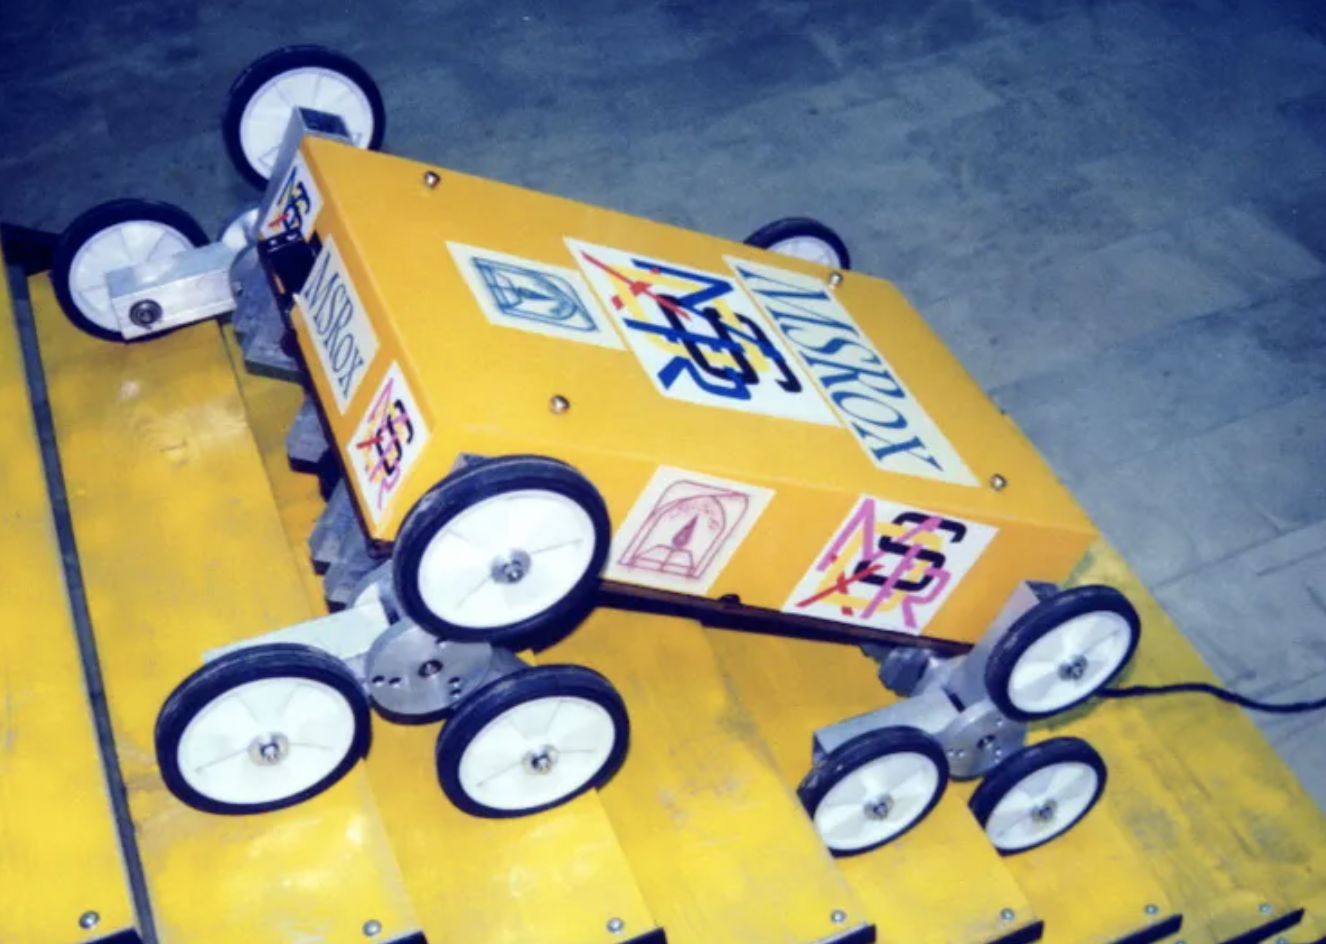
\includegraphics[width=0.45\linewidth]{../img/rox.png}
    \caption{Principe mécanique d’un système tri-star}
    \label{fig:tristar_schema}
\end{figure}
\subsubsection*{Auto-équilibrage: enjeux de contrôle et contraintes temps réel}

L’auto-équilibrage s’appuie sur le concept du pendule inversé: le robot est intrinsèquement instable et nécessite une correction continue. Les architectures de contrôle sont dites \textbf{sous-actionnées} (moins d’actionneurs que de degrés de liberté à maîtriser), ce qui accroît la complexité de stabilisation \cite{xin2025}. Le défi majeur est souvent la robustesse temps réel: variabilité du temps de calcul, concurrence entre tâches (capteurs, moteurs, communication) et sensibilité aux latences \cite{salwa2025}. La capacité à récupérer après perturbation (impact/choc) est un indicateur de performance clé.

\subsubsection*{Exemples de solutions d’auto-équilibrage}

Zhao et al. (2023) décrivent un robot d’inspection sur deux roues intégrant capteur 360° et gyroscope, capable de se stabiliser rapidement et de supporter une charge significative \cite{zhao2023}. Une approche alternative consiste à stabiliser via mécanismes physiques: Quaglia et al. (2011) présentent \textbf{Wheelchair.q}, fauteuil roulant motorisé avec capacité de franchissement et gestion du centre de masse via liaison à quatre barres, limitant le basculement lors de la montée \cite{quaglia2011}.
\begin{figure}[H]
    \centering
    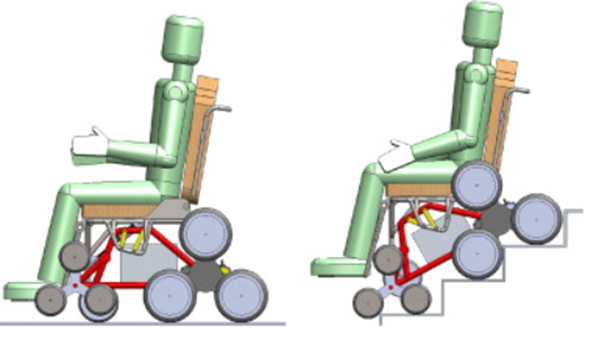
\includegraphics[width=0.45\linewidth]{../img/wheel.png}
    \caption{Modélisation du pendule inversé pour robot auto-équilibré}
    \label{fig:pendule_inverse}
\end{figure}
\subsection{Synthèse et positionnement de CarryBot}

L’état de l’art met en évidence deux axes structurants pour CarryBot:
\begin{itemize}
    \item \textbf{Logistique et assistance en environnement contrôlé} (clinique/domicile), avec fortes exigences de sécurité et d’acceptabilité.
    \item \textbf{Franchissement et stabilité}: la montée d’escaliers et le maintien de l’équilibre restent des défis techniques majeurs.
\end{itemize}

CarryBot se positionne comme un prototype académique orienté \textbf{transport d’objets légers en intérieur} et \textbf{franchissement d’irrégularités/marches faibles}, tout en priorisant une architecture simple, sécurisée et exploitable pédagogiquement.

% -------------------------------------------------------------
% 1.X ANALYSE DES BESOINS
% -------------------------------------------------------------
\section{Analyse des besoins}
\subsection{Analyse des besoins utilisateurs}

L’analyse des besoins repose sur une démarche centrée utilisateur visant à comprendre
les attentes, contraintes et usages possibles des futurs bénéficiaires du robot CarryBot.
Elle combine une approche qualitative (observations, entretiens exploratoires) et une
approche quantitative (questionnaire de caractérisation des besoins fonctionnels et
ergonomiques).\\

Les éléments identifiés mettent en évidence des exigences convergentes:

\begin{itemize}
    \item \textbf{Besoin d’assistance au transport d’objets du quotidien}  
    (médicaments, documents, bouteille d’eau, télécommande, petit matériel personnel).

    \item \textbf{Attente d’un robot simple à piloter}, notamment pour les utilisateurs présentant
    des limitations motrices ou cognitives: interface à pictogrammes, commandes limitées,
    retour visuel clair.

    \item \textbf{Sécurité en environnement intérieur}: arrêt immédiat, déplacement stable,
    absence de mouvements brusques.

    \item \textbf{Contrôle manuel prioritaire}: les utilisateurs souhaitent décider de la trajectoire
    et des actions du robot sans dépendre d’une autonomie complexe.

    \item \textbf{Franchissement d’obstacles simples}: seuils de portes, légères irrégularités,
    petites marches de quelques centimètres.

    \item \textbf{Faible effort cognitif}: la prise en main doit être immédiate.

    \item \textbf{Fonctionnement silencieux et non intrusif}: les usagers refusent tout robot
    perturbant l’environnement ou générant du stress.\\
\end{itemize}

Cette analyse confirme la pertinence d’un robot \emph{mobile, compact, stable, simple et
compréhensible}, conçu pour des environnements intérieurs restreints (chambre,
couloir, salle de rééducation, domicile adapté).


% -------------------------------------------------------------
% 1.X QUESTIONNAIRE UTILISATEUR
% -------------------------------------------------------------
\subsection{Formulaire d’analyse des besoins}

\begin{table}[H]
\centering
\renewcommand{\arraystretch}{1.5}
\setlength{\tabcolsep}{6pt}
\begin{tabular}{|p{4.5cm}|p{10.5cm}|}
\hline
\rowcolor{gray!15}
\textbf{Catégorie} & \textbf{Questions / Éléments à renseigner} \\
\hline

\textbf{Profil utilisateur} &
\begin{itemize}
    \item Âge?
    \item Situation (domicile, EHPAD, hôpital):
    \item Handicap moteur ou cognitif (oui/non, précisions):
    \item Niveau d’autonomie:
\end{itemize}
\\
\hline

\textbf{Usage prévu du robot} &
\begin{itemize}
    \item Besoin d’aide pour transporter des objets du quotidien? (oui/non)
    \item Objets à transporter principalement:
    \item Fréquence d’utilisation estimée:
    \item Lieux d’usage (chambre, salon, couloir, rééducation…):
\end{itemize}
\\
\hline

\textbf{Accessibilité} &
\begin{itemize}
    \item Préférence pour une interface avec pictogrammes? (oui/non)
    \item Difficultés avec smartphone ou tablette? (oui/non)
    \item Besoin d’un retour vocal? (oui/non)
    \item Besoin de commandes simplifiées? (oui/non)
\end{itemize}
\\
\hline

\textbf{Sécurité} &
\begin{itemize}
    \item Importance d’un bouton d’arrêt d’urgence? (faible/moyenne/élevée)
    \item Inquiétude face aux collisions ou mouvements brusques? (oui/non)
    \item Sensibilité à l’équilibre des objets transportés? (oui/non)
\end{itemize}
\\
\hline

\textbf{Fonctionnalités attendues} &
\begin{itemize}
    \item Arrêt du robot via l’application? (oui/non)
    \item Capacité à franchir de petites marches? (oui/non)
    \item Palette stabilisée/ajustable? (oui/non)
    \item Retour sonore (feedback)? (oui/non)
\end{itemize}
\\
\hline

\textbf{Observations complémentaires} &
Zone libre pour remarques, besoins spécifiques, contraintes particulières. \\ 
\hline

\end{tabular}
\caption{\small Formulaire synthétique d’analyse des besoins utilisateurs — Projet CarryBot}
\end{table}


% -------------------------------------------------------------
% 1.X PERSONAS
% -------------------------------------------------------------

\subsection{Personas — Public cible}

Les personas suivants représentent des profils-types construits à partir des besoins
identifiés. Ils servent de référence pour orienter la conception fonctionnelle et
ergonomique de CarryBot.

% Persona 1 -----------------------------------------------------
\begin{figure}[H]
    \centering
    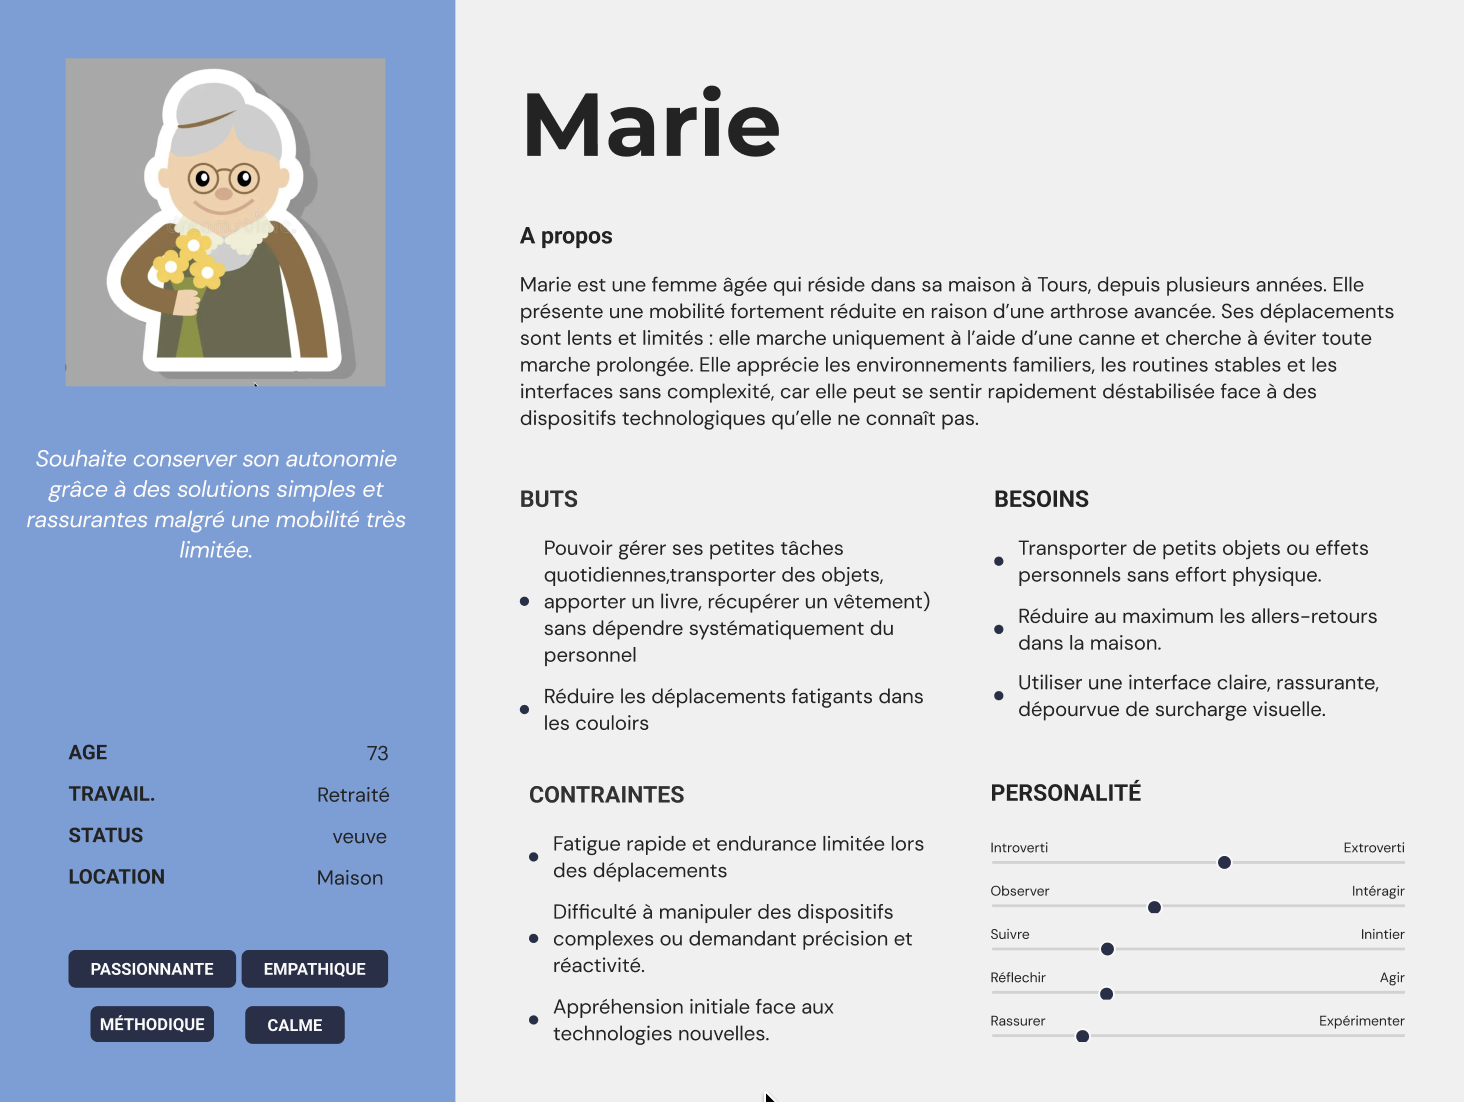
\includegraphics[width=0.6\textwidth]{../img/marie.png}
    \caption{Persona 1: Marie, 75 ans, retraitée}

\end{figure}

% Persona 2 -----------------------------------------------------
\begin{figure}[H]
    \centering
    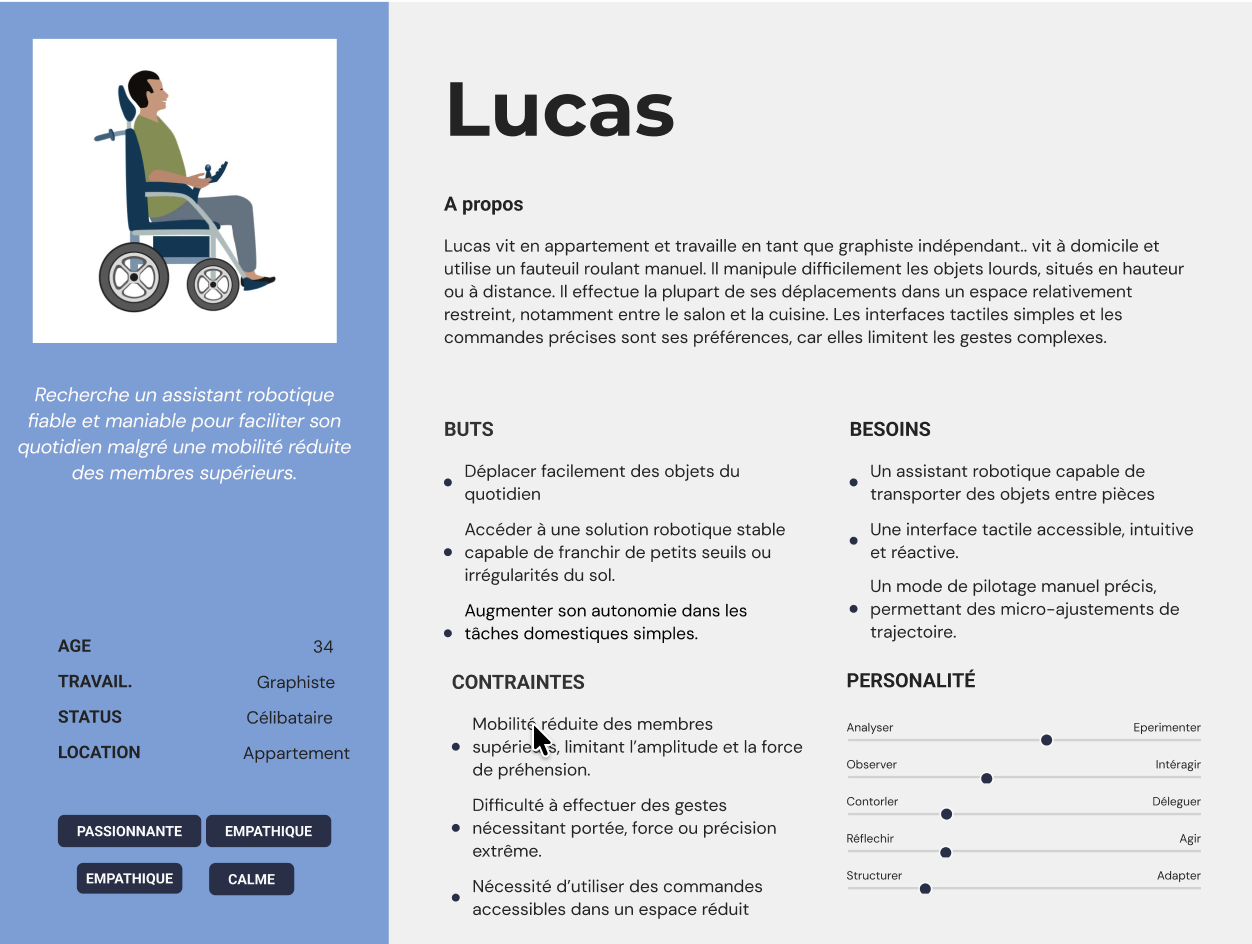
\includegraphics[width=0.6\textwidth]{../img/lucas.png}
    \caption{Persona 2: Lucas, 30 ans, à mobilité réduite}
\end{figure}

% -------------------------------------------------------------
% 4. EXIGENCES
% -------------------------------------------------------------
\section{Exigences}
\subsection{Exigences fonctionnelles}

\begin{tabular}{|p{1.3cm}|p{6.6cm}|p{1.7cm}|p{4,5cm}|}
\hline
\textbf{Id} & \textbf{Exigence} & \textbf{Priorité} & \textbf{Commentaire} \\ \hline


EF1 & Commande manuelle via application Android & H & Interface à pictogrammes simplifiée. \\ \hline

EF2 & Arrêt d’urgence physique & H & Interruption immédiate des moteurs. \\ \hline

EF3 & Arrêt logiciel sécurisé & H & Arrêt critique déclenché depuis l’application. \\ \hline

EF4 & Franchissement de petites marches & M & Système de roues Tri-Star. \\ \hline

EF5 & Transport d’objets légers sur palette motorisée & H & Capacité de charge jusqu’à 2 kg. \\ \hline

EF6 & Élévation de la palette motorisée & M & Transport d’objets légers. \\ \hline


\end{tabular}

\vspace{0.6cm}

\subsection{Exigences qualité (non fonctionnelles)}

\begin{tabular}{|p{1.3cm}|p{6.6cm}|p{1.7cm}|p{4.5cm}|}
\hline
\textbf{Id} & \textbf{Critère de qualité} & \textbf{Priorité} & \textbf{Commentaire} \\ \hline

EQ1 & Sécurisation du système & H & Gestion fiable des arrêts d’urgence. \\ \hline

EQ2 & Ergonomie de l’interface & H & Accessibilité UI, contraste, pictogrammes. \\ \hline

EQ3 & Robustesse mécanique & M & Résistance des composants imprimés 3D. \\ \hline

EQ4 & Autonomie minimale & M & 5 heures de fonctionnement continu. \\ \hline

\end{tabular}

\vspace{0.6cm}

\subsection{Exigences légales et réglementaires}

\begin{tabular}{|p{1.3cm}|p{6.6cm}|p{1.7cm}|p{4,5cm}|}
\hline
\textbf{Id} & \textbf{Exigence} & \textbf{Priorité} & \textbf{Commentaire} \\ \hline

EL1 & Conformité électrique & H & Respect des normes basse tension. \\ \hline

EL2 & Accessibilité numérique & H & Référentiel RGAA applicable à l’application mobile. \\ \hline

EL3 & Sécurité d’usage & M & Gestion des risques pour utilisateurs fragiles. \\ \hline

\end{tabular}

% -------------------------------------------------------------
% 3. DESCRIPTION DU SYSTEME
% -------------------------------------------------------------
\section{Description du système ou produit}
\subsection{Domaine couvert et périmètre du projet}

\subsubsection{Domaine couvert}
Le projet CarryBot couvre les domaines suivants:
\begin{itemize}
    \item \textbf{robotique mobile légère} en environnement intérieur;
    \item \textbf{interaction homme--robot accessible}, via une interface mobile simplifiée;
    \item \textbf{technologies embarquées} basées sur Raspberry~Pi et capteurs associés;
    \item \textbf{aide au transport d’objets} pour un usage domestique ou pédagogique;
    \item \textbf{conception d’un prototype fonctionnel} intégrant mécanique, électronique et logiciel.
\end{itemize}

\subsubsection{Périmètre du projet}
Le périmètre retenu inclut:
\begin{itemize}
    \item la mise en place d’un robot capable de se déplacer en intérieur;
    \item l’intégration d’une palette motorisée pour transporter de petits objets;
    \item la détection d’obstacles à courte distance;
    \item l’intégration de boutons d’arrêt d’urgence;
    \item le développement d’une application mobile pour le pilotage manuel;
    \item l’assemblage d’une architecture complète: mécanique, électronique et supervision logicielle.
\end{itemize}

\subsubsection{Hors périmètre}
Les fonctionnalités suivantes sont exclues de ce prototype:
\begin{itemize}
    \item \textbf{navigation autonome avancée} (SLAM, cartographie, planification complexe);
    \item \textbf{déplacements extérieurs} ou sur terrains non stabilisés;
    \item \textbf{transport de charges lourdes} ou applications industrielles;
    \item intégration de systèmes de \textbf{communication en réseau étendue} (IoT, cloud).
\end{itemize}

\vspace{0,5cm}
\subsection{Architecture}
L’architecture de CarryBot repose sur une intégration cohérente entre l’électronique embarquée, la motorisation, les systèmes de détection et la couche logicielle de supervision. Elle se structure comme suit:

% -------------------------------------------------------------
% Première rangée: deux photos côte à côte
% -------------------------------------------------------------
\begin{figure}[H]
    \centering
    \begin{minipage}{0.48\linewidth}
        \centering
        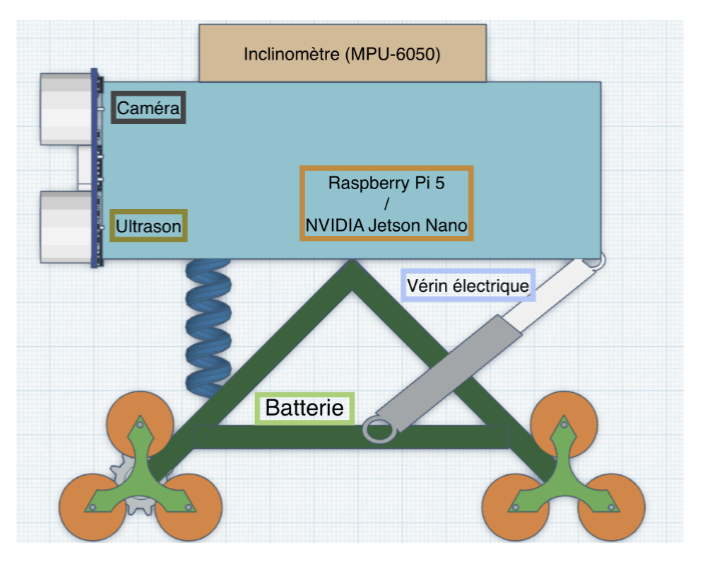
\includegraphics[width=\linewidth]{../img/CB-global.png}
        \caption{CarryBot en vue globale}
    \end{minipage}
    \hfill
    \begin{minipage}{0.48\linewidth}
        \centering
        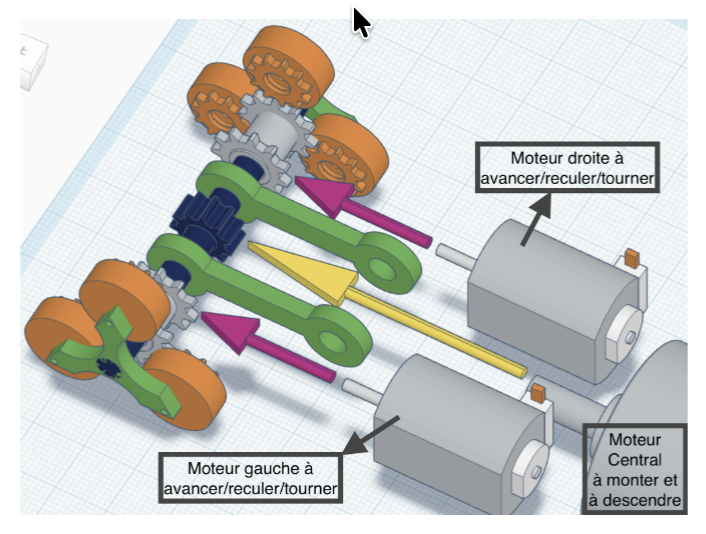
\includegraphics[width=\linewidth]{../img/CB-detail.png}
        \caption{Détail de la motorisation et des roues Tri-Star}
    \end{minipage}
\end{figure}


% -------------------------------------------------------------
% Deuxième rangée: deux photos côte à côte
% -------------------------------------------------------------
\begin{figure}[H]
    \centering
    \begin{minipage}{0.48\linewidth}
        \centering
        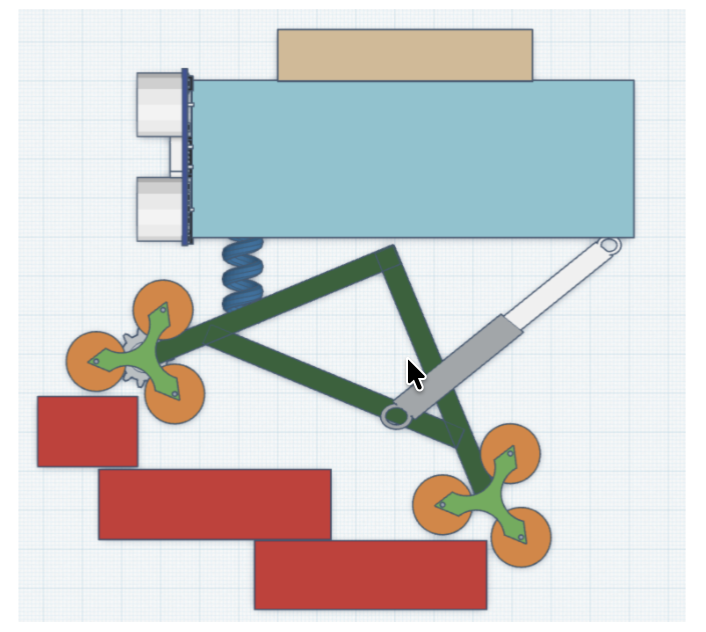
\includegraphics[width=\linewidth]{../img/monter.png}
        \caption{La montée de la palette motorisée}
    \end{minipage}
    \hfill
    \begin{minipage}{0.48\linewidth}
        \centering
        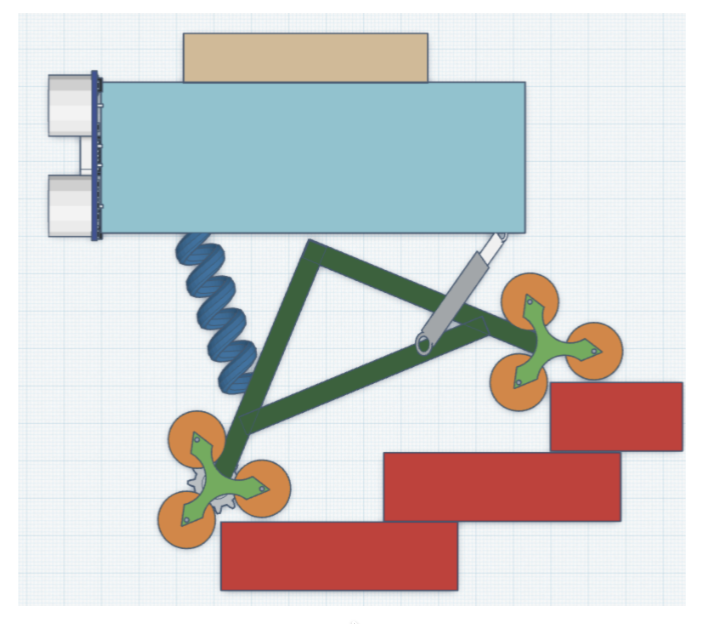
\includegraphics[width=\linewidth]{../img/descente.png}
        \caption{La descente de la palette motorisée}
    \end{minipage}
\end{figure}




\subsection{Matériel}
\begin{itemize}
    \item \textbf{Carte principale:} Raspberry Pi 5 (8\,GB), équipée d’une carte microSD 32\,GB, d’un refroidisseur \textit{Active Cooler} et d’un câble d’extension GPIO 40\,broches.
    \item \textbf{Caméra de perception:} Intel RealSense D435 pour la capture de profondeur et la détection avancée de l’environnement.
    \item \textbf{Capteurs ultrason:} 4 modules pour la détection d’obstacles à courte distance.
    \item \textbf{Unité inertielle (IMU):} module inclinomètre / accéléromètre / gyroscope (Makeblock) pour la mesure de l’inclinaison et la stabilisation.
    \item \textbf{Roues Tri-Star:} 20 roues (14 à l’avant, 6 à l’arrière) (Makeblock), imprimées en 3D, adaptées au franchissement de petites marches et irrégularités.
    \item \textbf{Motorisation:} 4 moteurs à courant continu (185\,RPM, 9\,V) assurant propulsion et direction.
    \item \textbf{Actionneur:} vérin linéaire électrique 12\,V, piloté via un module L293N pour l’élévation et la stabilisation de la plateforme.
    \item \textbf{Module UPS d’alimentation embarqué:} Le système est équipé d’un module UPS 5.1 V / 5 A conçu pour le Raspberry Pi 5, assurant une alimentation continue même en l’absence de source externe. Il supporte jusqu’à quatre accus 18650 montés en configuration adaptée pour une autonomie accrue. Il gère la charge, la décharge et le basculement automatique entre alimentation externe et batterie.
    \item \textbf{Sécurité:} 2 boutons d’arrêt d’urgence LetMeKnow permettant l’interruption immédiate de la puissance moteur.
\end{itemize}


\begin{figure}[H]
    \centering
    \begin{minipage}{0.37\linewidth}
        \centering
        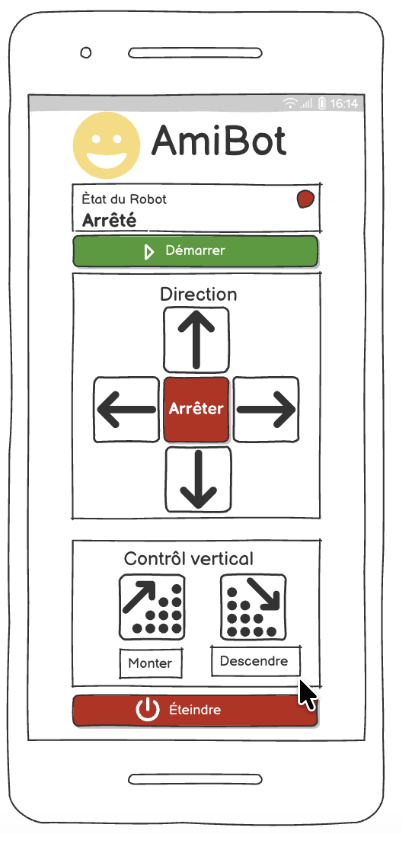
\includegraphics[width=\linewidth]{../img/appli-figma.png}
        \caption{Prototype Figma}
    \end{minipage}
    \hfill
    \begin{minipage}{0.37\linewidth}
        \centering
        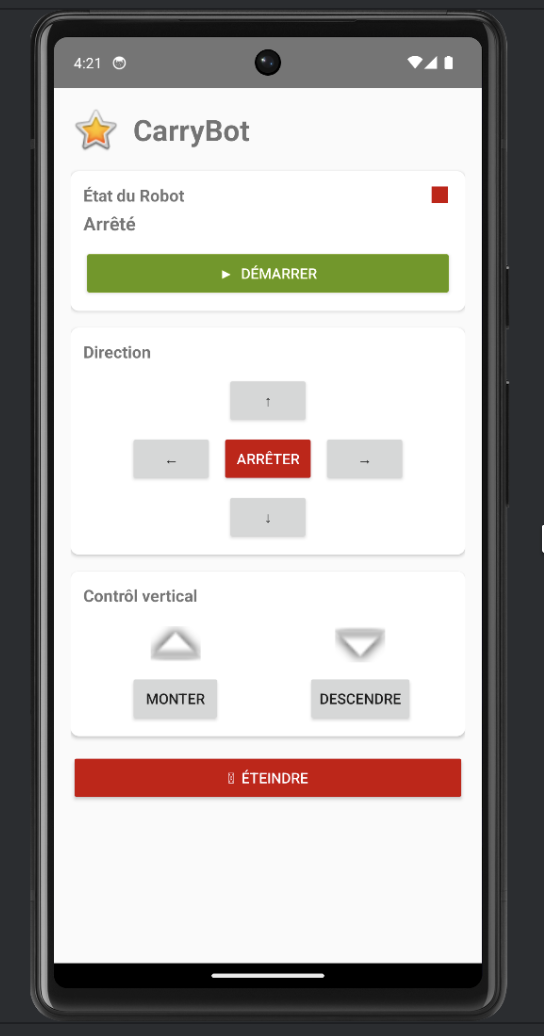
\includegraphics[width=\linewidth]{../img/appli-and.png}
        \caption{interface application Android}
    \end{minipage}
    \caption{Interface principale de l’application CarryBot}
    \label{fig:carrybot_series1}
\end{figure}

\subsection{Logiciel}
\begin{itemize}
    \item \textbf{Programme embarqué Raspberry Pi:} développé en Python ou C++, assurant:
    \begin{itemize}
        \item la gestion centrale de la motorisation,
        \item la fusion des données issues des capteurs (ultrason, IMU, caméra),
        \item la supervision de l’état du robot,
        \item la communication avec l’application mobile.
    \end{itemize}

    \item \textbf{Application Android:} développée sous Android Studio en Java, intégrant une interface à pictogrammes et des fonctionnalités d’accessibilité.
    
    \item \textbf{Microcontrôleurs additionnels (si requis):} gestion dédiée des capteurs ou actionneurs via interfaces GPIO ou bus série, en communication avec la Raspberry Pi.
\end{itemize}


%-------------------------------------------------------------


\subsection{Acteurs}

\begin{itemize}
    \item \textbf{Personnes à mobilité réduite (PMR)}: utilisateurs finaux susceptibles d’utiliser CarryBot pour transporter de petits objets et réduire les déplacements physiques.

    \item \textbf{Personnes âgées}: utilisateurs pouvant bénéficier d’un soutien pour limiter les efforts, prévenir les chutes et faciliter la manipulation d’objets en intérieur.

    \item \textbf{Patients en milieu hospitalier ou en centre de rééducation}: utilisateurs potentiels ayant besoin d’une aide pour déplacer des objets personnels, consommables ou équipements légers.

    \item \textbf{Aidants, infirmiers et personnels soignants}: acteurs susceptibles d’utiliser CarryBot comme outil d’assistance pour diminuer la charge physique liée à la manutention de matériel léger.

\end{itemize}
\vspace{0.5cm}

\noindent
\textit{À ce stade du projet, ces acteurs ne sont pas encore mis en relation directe avec le prototype.  
L’interaction effective avec CarryBot est actuellement limitée aux membres de l’équipe projet pour les activités de conception, de test et de validation interne.}


% -------------------------------------------------------------
% 4. SOLUTIONS ET ORIENTATIONS
% -------------------------------------------------------------
\section{Solutions et orientations}

\subsection{Solutions techniques retenues}

\begin{itemize}
    \item \textbf{Pilotage manuel via application Android}:
    contrôle directionnel simple, interface à pictogrammes et options d’accessibilité.

    \item \textbf{Franchissement de petites marches}:
    roues Tri-Star pour seuils et marches de faible hauteur.

    \item \textbf{Stabilisation de la charge}:
    plateau assisté par vérin pour maintenir les objets lors des franchissements.

    \item \textbf{Sécurité}:
    arrêt d’urgence physique et arrêt logiciel depuis l’application.

    \item \textbf{Feedback utilisateur}:
    retours visuels (états) et option de retour vocal.
\end{itemize}

%--------------------------------------------------------------
\subsection{Contraintes et orientations de conception}

\begin{itemize}
    \item \textbf{Contraintes physiques}: masse totale du robot inférieure à 3~kg.
    \item \textbf{Contraintes d’autonomie}: le robot est alimenté via un module UPS 5.1 V / 5 A compatible Raspberry Pi 5, utilisant jusqu’à quatre cellules 18650. L’autonomie dépend du nombre et de la capacité des cellules installées, mais le système assure une alimentation stable pour la durée des essais prévus.
    \item \textbf{Contraintes de sécurité}: mécanismes d’arrêt d’urgence adaptés à un usage hospitalier et PMR.
\end{itemize}

%-------------------------------------------------------------
\subsection{Perspectives d’évolution}

\begin{itemize}
    \item \textbf{Mode semi-autonome par suivi de bande au sol} (non implémenté):
    navigation assistée sur trajectoires prédéfinies, réduction de charge cognitive, usage pertinent en environnements structurés.

    \item \textbf{Suivi de personne}:
    assistance mobile au déplacement (cas aidant / clinique).

    \item \textbf{Cartographie et localisation}:
    intégration potentielle LIDAR/SLAM selon maturité technique.

    \item \textbf{Version industrialisable}:
    motorisation plus coupleuse, châssis renforcé, autonomie accrue.
\end{itemize}

% -------------------------------------------------------------
% 5. VALIDATION UTILISATEURS
% -------------------------------------------------------------
\section{Validation et tests utilisateurs}

\subsection{Critères de validation — Tests techniques et fonctionnels}

L’évaluation du prototype CarryBot repose sur plusieurs indicateurs techniques mesurables:

\textbf{Autonomie:} durée de fonctionnement avant recharge de la batterie, mesurée en minutes. Pour le prototype actuel, l’objectif minimal est de 5 heures en fonctionnement continu. Une optimisation future visera une autonomie significativement plus élevée.

\textbf{Vitesse de déplacement horizontal:} mesurée en mètres par seconde. Une attention particulière est portée à la fluidité des virages et à la stabilité lors des changements de direction.

\textbf{Capacité de déplacement vertical:} nombre de marches franchissables consécutivement. Le prototype actuel permet le franchissement de marches d’environ 4 cm. L’objectif minimal est de franchir trois marches successives.

\textbf{Capacité de charge:} transport sécurisé d’objets légers (jusqu’à 2 kg dans la version actuelle).

\textbf{Efficacité du rééquilibrage:} capacité du système à détecter une inclinaison du plateau et à rétablir l’horizontalité via le vérin:
\begin{itemize}
    \item Temps de stabilisation (objectif initial: < 2 secondes)
    \item Maintien des objets sans chute ni dégradation
\end{itemize}

\textbf{Détection d’obstacles:} capacité à identifier des éléments fixes (murs, escaliers, mobilier) afin d’éviter les collisions.

\textbf{Contrôle manuel:} réactivité et précision des commandes envoyées depuis l’application Android.

\textbf{Ergonomie de l’application:} évaluation selon les critères de Bastien et Scapin, et conformité aux principes d’accessibilité (RGAA).

\newpage

% -------------------------------------------------------------
% -------------------------------------------------------------
\subsection{Scénario UX 1 — Personne à Mobilité Réduite (PMR)}

Lucas, 30 ans, vit dans une maison à deux étages adaptée à son fauteuil roulant. Il utilise CarryBot comme dispositif d’assistance pour transporter des objets essentiels entre les niveaux de son domicile.

Ce matin, installé dans sa chambre à l’étage, Lucas souhaite récupérer ses médicaments laissés au rez-de-chaussée dans le compartiment du robot. Plutôt que de descendre immédiatement, il décide d’utiliser CarryBot.

Il ouvre l’application mobile. L’interface propose un mode unique de pilotage manuel, avec des commandes directionnelles simples (avant, arrière, gauche, droite, montée).

Lucas dirige le robot depuis le rez-de-chaussée vers l’escalier. Une fois positionné correctement, il active la commande de montée. Le robot entame l’ascension de manière contrôlée. L’application affiche un retour d’état : “Montée en cours”.

Lucas observe la progression. La stabilisation du plateau s’active automatiquement pour maintenir les objets à niveau. Arrivé à l’étage, Lucas reprend le contrôle directionnel pour guider CarryBot jusqu’à sa chambre.

Le robot s’arrête devant lui. Lucas ouvre le compartiment, récupère ses médicaments, puis pilote le robot pour le renvoyer au rez-de-chaussée.

L’interaction reste simple, directe et maîtrisée : l’utilisateur conserve le contrôle total du déplacement, ce qui renforce la sensation de sécurité et de fiabilité.

\subsubsection*{Questionnaire utilisateur — Scénario Lucas}

\textbf{1 — Compréhension et ergonomie}
\begin{itemize}
    \item Les commandes directionnelles sont-elles intuitives ?
    \item Les icônes sont-elles claires et facilement identifiables ?
    \item L’interface vous semble-t-elle adaptée à un usage quotidien ?
    \item Les retours d’état (montée, arrêt, obstacle) sont-ils compréhensibles ?
\end{itemize}

\textbf{2 — Performance du robot}
\begin{itemize}
    \item Le robot répond-il rapidement aux commandes ?
    \item Le déplacement est-il suffisamment fluide ?
    \item La montée des marches vous paraît-elle stable ?
    \item Vous sentez-vous en confiance lors du pilotage manuel ?
    \item Le transport des objets est-il sécurisé ?
\end{itemize}


% -------------------------------------------------------------
% DISCUSSION / LIMITES
% -------------------------------------------------------------
\section{Discussion, limites et axes d’amélioration}

Le prototype CarryBot a permis de valider une partie des choix de conception (intégration mécanique, architecture embarquée, pilotage via application, sécurisation par arrêt d’urgence). Néanmoins, plusieurs limites ont été identifiées lors des essais et de l’intégration finale.

\subsection{Limites observées}

\begin{itemize}
    \item \textbf{Motorisation insuffisante :} les moteurs utilisés se sont révélés trop faibles au regard des contraintes dynamiques (friction, couple requis, variations de charge, franchissement). Cette limite impacte directement la fiabilité du déplacement et la capacité à maintenir un comportement stable dans des situations exigeantes.
    \item \textbf{Navigation semi-autonome non intégrée :} le suivi de ligne automatique initialement prévu n’a pas pu être implémenté faute de temps. Le prototype final se limite donc à un \textbf{pilotage manuel supervisé}.
    \item \textbf{Marge de progression sur la robustesse d’intégration :} la stabilité globale (câblage, maintien mécanique, tolérances d’impression 3D, qualité de contact au sol) peut être améliorée pour augmenter la répétabilité des tests et réduire les dérives comportementales.
\end{itemize}

\subsection{Améliorations prioritaires}

\begin{itemize}
    \item \textbf{Re-dimensionnement de la motorisation :} choix de moteurs plus coupleux, optimisation des rapports de réduction, et calibration de l’alimentation (tension/courant) en cohérence avec la charge et les pentes à franchir.
    \item \textbf{Optimisation mécanique :} réduction des pertes (friction/jeu), renforcement des pièces sollicitées, amélioration de la géométrie et de la répartition des masses (centre de gravité).
    \item \textbf{Intégration du suivi de ligne :} implémentation d’un mode semi-autonome (capteurs + logique de contrôle), avec stratégie de sécurité (arrêt en cas de perte de trace / obstacle) et protocole de validation.
    \item \textbf{Montée en maturité des tests :} scénarios de test standardisés, métriques reproductibles (vitesse, couple, autonomie, stabilité), et journalisation (logs) pour analyser les défaillances.
\end{itemize}

\subsection{Conclusion opérationnelle}

CarryBot constitue un démonstrateur pertinent sur le plan pédagogique et technique. Les résultats mettent en évidence des verrous concrets (notamment la puissance moteur et la non-intégration de la navigation semi-autonome) qui structurent clairement la feuille de route d’industrialisation du prototype.

%-------------------------------------------------------------
% RÉFÉRENCES
%-------------------------------------------------------------
\newpage

\section*{Bibliographie}
\begin{thebibliography}{99}
\bibitem{rosa}
Hospital News, "How ROSA the Robot Will Help Isolated Seniors and Support Aging in Place", 2022. 
\url{https://hospitalnews.com/how-rosa-the-robot-will-help-isolated-seniors-and-support-aging-in-place/}
\bibitem{labrador}
Labrador Systems, "Labrador Retriever", 2022.  \url{https://labradorsystems.com/}
\bibitem{helpe} Borobo, "Help-E", 2022. \url{https://borobo.fr/}\\

\bibitem{bloss2011}
Bloss, R. (2011). Mobile hospital robots cure numerous logistic needs. \textit{Industrial Robot}, 38(6), 567--571. https://doi.org/10.1108/01439911111179075

\bibitem{bourdon2023}
Bourdon, J. (2023). Rethinking telepresence: post- and pre-COVID-19. \textit{Media, Culture \& Society}, 45(4), 884--895. https://doi.org/10.1177/01634437231159527

\bibitem{teng2022}
Teng, R., Ding, Y., \& See, K.C. (2022). Use of Robots in Critical Care: Systematic Review. \textit{JMIR}, 24(5), e33380. https://doi.org/10.2196/33380

\bibitem{wang2024}
Wang, B., Chen, S., \& Xiao, G. (2024). Advancing healthcare through mobile collaboration: a survey of intelligent nursing robots research. \textit{Frontiers in Public Health}, 12, 1368805. https://doi.org/10.3389/fpubh.2024.1368805

\bibitem{holland2021}
Holland, J., Kingston, L., McCarthy, C., et al. (2021). Service Robots in the Healthcare Sector. \textit{Robotics}, 10(1), 47. https://doi.org/10.3390/robotics10010047

\bibitem{graf2009}
Graf, B., Parlitz, C., \& H\"agele, M. (2009). Robotic Home Assistant Care-O-bot\textsuperscript{\textregistered}~3 Product Vision and Innovation Platform. In \textit{HCI 2009, LNCS 5611}. \url{https://doi.org/10.1007/978-3-642-02577-8_34}

\bibitem{graf2023}
Graf, B., \& Eckstein, J. (2023). Service Robots and Automation for the Disabled and Nursing Home Care. In \textit{Springer Handbook of Automation}. \url{https://doi.org/10.1007/978-3-030-96729-1_62}

\bibitem{kittmann2015}
Kittmann, R., Fröhlich, T., Schäfer, J., et al. (2015). Let me Introduce Myself: I am Care-O-bot 4, a Gentleman Robot. In \textit{Mensch und Computer 2015}. https://doi.org/10.1515/9783110443929-024

\bibitem{li2023}
Li, S., Milligan, K., Blythe, P., et al. (2023). Exploring the role of human-following robots in supporting the mobility and wellbeing of older people. \textit{Scientific Reports}, 13, 6512. https://doi.org/10.1038/s41598-023-33837-1

\bibitem{shibata2011}
Shibata, T., \& Wada, K. (2011). Robot therapy: a new approach for mental healthcare of the elderly--a mini-review. \textit{Gerontology}, 57(4), 378--386.

\bibitem{seo2023}
Seo, T., Ryu, S., Won, J.H., Kim, Y., \& Kim, H.S. (2023). Stair-Climbing Robots: A Review on Mechanism, Sensing, and Performance Evaluation. \textit{IEEE Access}, 11, 60539--60561. https://doi.org/10.1109/ACCESS.2023.3286871

\bibitem{dalvand2006}
Dalvand, M.M., \& Moghadam, M.M. (2006). Stair Climber Smart Mobile Robot (MSRox). \textit{Autonomous Robots}, 20, 3--14. https://doi.org/10.1007/s10514-006-5364-4

\bibitem{salwa2025}
Salwa, M., \& Krzysztofik, I. (2025). Influence of Control System Architecture on Mobile Robot Stability and Performance. \textit{Sensors}, 25(23), 7353. https://doi.org/10.3390/s25237353

\bibitem{xin2025}
Xin, G., Jin, B., Liu, C., \& Jiang, M. (2025). A Unified Control Framework for Self-Balancing Robots... \textit{Sensors}, 25(23), 7144. https://doi.org/10.3390/s25237144

\bibitem{zhao2023}
Zhao, J., Li, J., \& Zhou, J. (2023). Research on Two-Round Self-Balancing Robot SLAM... \textit{Sensors}, 23(5), 2489. https://doi.org/10.3390/s23052489

\bibitem{quaglia2011}
Quaglia, G., Franco, W., \& Oderio, R. (2011). Wheelchair.q, a motorized wheelchair with stair climbing ability. \textit{Mechanism and Machine Theory}, 46(11), 1601--1609. https://doi.org/10.1016/j.mechmachtheory.2011.07.005

\end{thebibliography}

\end{document}
